\documentclass{article}


%help
%https://www.latex-tutorial.com/tutorials/beginners/how-to-use-latex/
%https://en.wikibooks.org/wiki/LaTeX/Source_Code_Listings

%preamble
\usepackage[utf8]{inputenc}
\usepackage{amsmath}
\usepackage{graphicx}
\usepackage{booktabs}
\usepackage{listings}
\usepackage{color}
\usepackage{tikz}
\usepackage{hyperref}

\lstset{ %
  language=R,                     % the language of the code
  basicstyle=\footnotesize,       % the size of the fonts that are used for the code
  numbers=left,                   % where to put the line-numbers
  numberstyle=\tiny\color{gray},  % the style that is used for the line-numbers
  stepnumber=1,                   % the step between two line-numbers. If it's 1, each line
                                  % will be numbered
  numbersep=5pt,                  % how far the line-numbers are from the code
  backgroundcolor=\color{white},  % choose the background color. You must add \usepackage{color}
  showspaces=false,               % show spaces adding particular underscores
  showstringspaces=false,         % underline spaces within strings
  showtabs=false,                 % show tabs within strings adding particular underscores
  frame=single,                   % adds a frame around the code
  rulecolor=\color{black},        % if not set, the frame-color may be changed on line-breaks within not-black text (e.g. commens (green here))
  tabsize=2,                      % sets default tabsize to 2 spaces
  captionpos=b,                   % sets the caption-position to bottom
  breaklines=true,                % sets automatic line breaking
  breakatwhitespace=true,        % sets if automatic breaks should only happen at whitespace
  title=\lstname,                 % show the filename of files included with \lstinputlisting;
                                  % also try caption instead of title
  keywordstyle=\color{blue},      % keyword style
  commentstyle=\color{green},   % comment style
  stringstyle=\color{purple},      % string literal style
  escapeinside={\%*}{*)},         % if you want to add a comment within your code
  morekeywords={*,...}            % if you want to add more keywords to the set
}

\title{Bayesian statistics \\
\vskip 1cm
\Large Introduction to Bayesian methods in ecology and evolution}
\vskip 1cm
\author{Matteo Fumagalli \\ m.fumagalli@imperial.ac.uk \\ Imperial College London}




\begin{document}

	\pagenumbering{gobble}
	\maketitle

	\newpage

	\tableofcontents
	\newpage
	\pagenumbering{arabic}

	
\section{Birds}

        You are in the Galapagos and you want to model the distribution of beak widths in
        Darwin finches.
        In the species you are investigating, you know my past information that this width is
        very different between sexes but highly homogenous within each sex (there is no much
        variation in beak width within each sex).
        In particular experts told you that the average beak width for males is 12mm while the
        average width for females is 25mm.
        You also know that in the particular island you are located the proportion of females vs. males
        is $\frac{3}{2}$.

        \paragraph{Question A}

        Based on this piece of information, propose a suitable prior distribution on the
        parameter beak width assuming that you are interested in describing the beak width in the
        entire population (both sexes comprised) in the island where you are located.
        Hint: imagine you randomly pick one bird, what is the expected beak width?

        \paragraph{Question B}

        Let's suppose you move to another island, which is still unexplored, and you want to investigate
        the beak width, $\theta$, of female birds only.
        You collect $n=10$ samples and your likelihood function is $N(\theta | \mu,\sigma^2)$
        and 25 is the average value across the 10 samples with a variance of 5.

        What are the appropriate values for $\mu$ and $\sigma^2$?

	\paragraph{Question C}

        You now want to derive a posterior distribution
        for $\theta$. You ask for prior information from four different experts (Dr Harrison, Dr Lennon,
        Dr McCartney, Dr Starr). Based on each prior distribution suggested, you obtained the following
        posterior distributions.

        \begin{figure}[!ht]
                \centering
                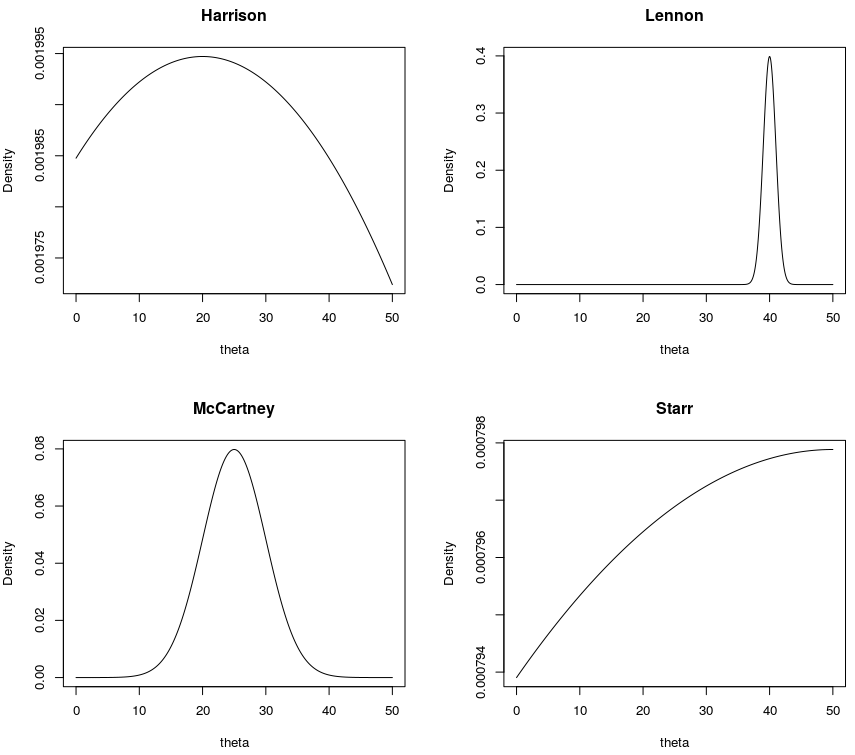
\includegraphics[width=10cm]{Figures/test.png}
                \caption{Posterior distributions for Question C on birds.}
        \end{figure}

        Discuss which prior might be more suitable in the case where: (i) you have little idea on what to expect
        in this new island for your parameter or (ii) expect that the beak width is comparable to what known
        in the previous island (as in Question A).
        Discuss one point for each posterior (e.g. who is the most or least confident, who uses a safest or
        bravest prior, etc ect.).

	\paragraph{Question D}

        You want to study another character, the beak length $\theta_2$ which is correlated with
        the beak width, now labelled $\theta_1$. Your vector of parameters is now
        $\vec{\theta}=\{\theta_1, \theta_2\}$.
        You choose a uniform prior (not conjugate to the Normal distrbution) and therefore choose
        an MCMC algorithm (specifically the Metropolis algorithm) to obtain samples from the
        posterior distribution.

        The algorithm begins by proposing a \textit{proposal} symmetric density
        $q(\vec{\theta}^* | \vec{\theta}^{(t-1)})$ which satisfies
        $q(\vec{\theta}^* | \vec{\theta}^{(t-1)})=q(\vec{\theta}^{(t-1)} | \vec{\theta}^*)$.
        From a starting value $\vec{\theta^{(0)}}$ at iteration $t=0$, for $(t=1,..., T)$
        the algorithm repeats:
        \begin{enumerate}
                \item draw $\vec{\theta}^* = q( \cdot | \vec{\theta}^{(t-1)})$,
                \item calculate $r=h(\vec{\theta}^*)/h(\vec{\theta}^{(t-1)})$,
                \item if $r \geq 1$, set $\vec{\theta}^{(t)}=\vec{\theta}^*$, otherwise\\
                        set $\vec{\theta}^{(t)}=\vec{\theta}^*$ with probability $r$ or\\
                        set $\vec{\theta}^{(t)}=\vec{\theta}^{(t-1)}$ with probability $1-r$.
        \end{enumerate}
        Under mild assumptions, $\vec{\theta}^{(t)}$ converges in distribution to a draw
        from the true posterior density $p(\vec{\theta}|\vec{y})$.

        The samples obtained by this algorithm are auto-correlated, as the sampling at time $t$
        is conditional to the sampling at time $t-1$.
        This is often not entirely satisfactory as ideally we want to draw uncorrelated samples from the
        posterior distribution.
        Propose a modification of the algorithm written above (or write a pseudocode) to ensure that your
        samplings from the Markov chain are fairly uncorrelated.
        Discuss pros and cons of your modification.

 	Another issue in this computation is that $\theta_1$ and $\theta_2$ are highly correlated (or
        you expect them to be highly correlated).
        In this case the chain will have a "slow mixing" and may explore only a fraction of the parameter
        space.
        Propose a modification of the algorithm written above (or write a pseudocode) to ensure that
        you reach convergence (by exploring the whole parameter space) even for correlated parameters
        $\theta_1$ and $\theta_2$.
        Discuss pros and cons of your modification and suggest a computational technique to overcome
        a potential disadvantage of this modification (hint: assume you can use the HPC).









	
\section{Frogs}

        During your latest field trip in Costa Rica you observed how brightly coloured
        poison dart frogs (part of the \textit{Dendrobatidae} family) were.
        In fact, the brightness of their skin colouration is correlated with their toxicity.
        To investigate the prevalence of toxic frogs in the area under study, you collected
        $n$ samples of poison dart frogs and observed that $k$ of them have bright skin colour
        (and thus are toxic).

        \paragraph{Question A}

        You now want to estimate the \textbf{population} frequency of the red colour
        phenotype, $f \in [0,1]$.
        Assuming a generic likelihood function $p(k|f,n)$, where $k$ is our observed data,
        and prior distribution $p(f)$, write the expression for the posterior distribution
        of $f$, $p(f | n,k)$.
        Indicate the interval for the integration over $f$ explicitly.
        Finally, if $p(f|\mu)$ (assuming we have uncertainty on the prior for $f$
        with parameter $\mu$, what is the resulting full equation for the posterior
        distribution $p(f | n,k,\mu)$?

        \paragraph{Question B}

	If we define the likelihood function as a Binomial distribution:
        \begin{equation}
                p(k|f,n) = ( \genfrac{}{}{0pt}{}{n}{k} ) f^k(1-f)^{n-k}
        \end{equation}
        and the prior function as a Beta distribution $B(\alpha,\beta)$:
        \begin{equation}
                p(f) = \frac{1}{B(\alpha,\beta)} f^{\alpha-1}(1-f)^{\beta-1}
        \end{equation}
        then the posterior distribution of $f$ is a Beta distribution with
        parameters $\alpha'=k+\alpha$ and $\beta'=n-k+\beta$.

        What is the frequentist estimate of $f$?
        What is the maximum likelihood estimate of $f$?
        What is the maximum \textit{a posteriori} mode of $f$ using the noninformative
        conjugate prior $p(f) \sim B(\alpha=1,\beta=1)$?
        What is the maximum \textit{a posteriori} mode of $f$ assuming $k=12$ and $n=235$ using the
        uniform prior $p(f) \sim U(0.5,1)$?

        \paragraph{Question C}

        Assuming we collected 100 samples and 25 of them have bright skin colour,
        please complete the \texttt{R} code below in order to generate both the exact
        and approximated posterior distribution of $f$ using the informative
        prior $p(f) \sim B(\alpha=2,\beta=1)$.
        You need to fill in where the string '???' is present.
        Finally, discuss which summaries you would report to describe the resulting posterior
        distribution.
	\begin{lstlisting}[language=R]
                # we evaluate our parameter f over a grid of 100 values for the whole range [0,1]
                f <- seq(0, 1, ???)

                # suppose we collected 100 samples and 25 of them have bright skin colour
                k <- 25
                n <- 100
                # alpha and beta are the parameter values for the posterior Beta distribution
                alpha <- ???
                beta <- ???

                # we now evaluate the density function to obtain the EXACT posterior distribution
                y <- ???(???, shape1=alpha, shape2=beta)

                # we now use Monte Carlo sampling to obtain the APPROXIMATED posterior distribution.
                Make a reasonable choice for the number of random samples.
                y_sampled <- ???
                y_sampled_distribution <- ???

        \end{lstlisting}

        \paragraph{Question D}

	If we use a Normal distribution as prior information, such as
        $p(f)=N(\mu,\sigma^2)$, we cannot derive a closed form and cannot sample
        directly from the posterior distribution.
        We can use a rejection sampling algorithm for \textit{indirect} sampling of the
        posterior distribution.
        This algorithm requires the identification of an envelope function $g(f)$ and a
        constant $M>0$ such that $p(k|f,n)p(f)<Mg(f)$.

        Identify both a suitable envelope function $g(f)$ and a value for $M$ assuming that
        we know that the maximum density value for the posterior distribution is $K$.
        Describe the full algorithm (with formal notation for equarions, e.g. $\nu \sim P(\lambda=2)$)
        or write its pseudocode (as accurate as possible).
        Describe what happens to the algorithm and/or the approximation if we
        choose $M>>K$ or $M<<K$.

        If we want to use an MCMC sampling approach, is it possible to use a Gibbs sampler in this case
        or is it more appropriate to use a rejection algorithm like the Metropolis one? Why?




	
\section{Ancient DNA}

You are hiking on the Pyrenees mountain range and you discovered an ancient human bone.
You extracted the DNA and sequenced its genome.
Unfortunately the sample was not well preserved and it was highly contaminated.
Therefore you were able to obtain the genotypic information for only one locus.
Specifically, you found that, at a specific genomic position, the mysterious ancient human has an \texttt{AA} genotype, homozygous for adenine.
Nevertheless, you want to make some statistical inferences on whether this sample is genetically closer to modern Spanish, French or Basque individuals.
This analysis is a proxy for understanding whether this sample is more likely to be an ancestor for modern Spanish, French or Basque.
In other words, you want to perform a \textbf{population assignment} based on genetic data.

Let's assume that your parameter of interest is $\theta=\{S,F,B\}$ representing the probability that your sample comes from a Spanish (S), French (F) or Basque (B) population, respectively.
The data is $y=\{g, f_A^{(S)}, f_A^{(F)}, f_A^{(B)}\}$ where $g$ is the ancient genotype (so that $g=AA$) and $f_A^{(S)}$, $f_A^{(F)}$, $f_A^{(B)}$ are the known population frequencies of allele $A$ in modern Spanish, French and Basque, respectively.
Under the assumption of Hardy Weinberg Equilibrium, we know that
\begin{equation*}
p(g=AA, f_A^{(i)}|\theta=i)=(f_A^{(i)})^2
\end{equation*}
for a generic population $i$.
Note the latter equation represents the likelihood function $f(y|\theta)$.

\paragraph{Question A}

Using Bayes' law, write the equation for the posterior probability of the sample belonging to the Spanish population given the data. Assume that you have a generic prior probability $\pi(\theta)$ with known hyperparameters. Be as formal and explicit as possible. No proofs or extra calculations are required.
Let's assume that we gather the follow population allele frequencies
\begin{align*}
f_A^{(S)} &= 0.7\\
f_A^{(F)} &= 0.2\\
f_A^{(B)} &= 0.1\\
\end{align*}
and that we ask for an opinion to experts regarding a prior probability of this sample belonging to any of the tested populations.
Here the opinion from our 3 experts:
\begin{enumerate}
        \item Dr Cobain: \texttt{It is still highly debated whether ancient humans in the Pyrenees are the ancestors of modern French, Spanish or Basque. All anthropological evidences so far are not solid enough to point towards any specific population. We have no clue!}
    \item Professor Grohl FRS: \texttt{It must be Spanish. I see no evidence why this sample should be the ancestor of any other modern population. I am 100\% sure.}
    \item Mr Novoselic: \texttt{We have collected more than 1,000 ancient samples from Pyrenees so far and we were able to assign 50\% of them as Spanish, 30\% as French, and 20\% as Basque.}
\end{enumerate}

\paragraph{Question B}

Based on this information, choose the most suitable prior distribution $\pi(\theta)$. Justify your choice. There is no right or wrong answer (although one of them is hardly acceptable) as long as it is properly justified. Formalise $\pi(\theta)$ by assigning a prior probability for each value of $\theta$ based on your choice.

\paragraph{Question C}

Based on your chosen prior distribution, calculate the Bayes factor for model $M_1$ with parameter $\{\theta=S\}$ \textit{vs.} model $M_2$ with parameter $\{\theta \neq S\}$. Write the equation and provide the value for the Bayes factor. Approximate any calculation as much as you wish but be reasonable (e.g. $0.82/0.19 \approx 4$ is totally fine but $0.82/0.19 \approx 3$ is not). Provide a brief discussion on the support for $M_1$ or $M_2$.

\paragraph{Question D}

Let's assume that a new prior probability on $\theta$ is now dependent on an unknown hyperparameter $\tau$ with distribution $h(\tau)$ with $\tau=\{-1,0,1\}$. In other words, the prior distribution is $\pi(\theta|\tau)$ and $\tau$ can only have the discrete values of $-1$, $0$, or $-1$. Using Bayes' law in hierarchical modelling, write the equation for the posterior distribution of the sample being Spanish. Be as formal and explicit as possible. No proofs or extra calculations are required. Note that both $\theta$ and $\tau$ are discrete distributions.

Finally, you want to estimate the posterior distribution for the allele frequency of the ancestral Spanish population given the ancient and modern genotype data. Let's call this parameter $\phi$, continuous within the range $[0,1]$. The model is more complicated (and outside the scope of this exercise) and indeed you cannot derive a closed form for the posterior distribution. Therefore you want to use an indirect sampling method to approximate the posterior distribution $p(\phi|y)$.
As seen in class, one possibility is to use a \textit{rejection sampling} algorithm which uses an envelope function to "cover" the posterior distribution. However, this algorithm requires the specification of $M$ so that $L(\phi)\pi(\phi) < Mg(\phi)$ with $L(\phi)$ being the likelihood function. $M$ may be not readily available. Furthermore, this algorithm is computationally inefficient as it has a rejection step.

Therefore, you want to derive and implement a more efficient algorithm for indirect sampling of the posterior distribution, $p(\phi)$. Suppose you have $N$ draws of $\phi$ (so $\phi_1$, $\phi_2$, ...$\phi_N$) sampled from some approximating density function $g(\phi)$. This situation is illustrated in Figure \ref{fig:approx}. The continuous black line is the unknown posterior distribution, or a distribution up to a constant to $L(\phi)\pi(\phi)$; the red dashed line is the chosen approximating density $g(\phi)$; red small vertical lines on the x-axis represent the $N$ samples drawn which are then evaluated at $g(\phi)$.

\begin{figure}[h!]
        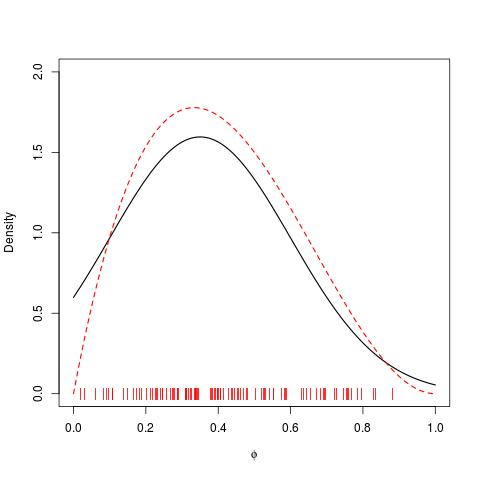
\includegraphics[width=0.9\textwidth]{Figures/sampling.jpeg}
	\caption{Indirect sampling to approximate a posterior distribution.}
    \label{fig:approx}
\end{figure}

\paragraph{Question E}

Assume that you can evaluate $L(\phi_i)\pi(\phi_i)$ and $g(\phi_i)$ for each one of the $N$ draws of $\phi$. You cannot sample from $L(\phi)\pi(\phi)$ but you can sample from $g(\phi)$ which is an approximating function for the posterior distribution. Devise an efficient algorithm for sampling $\phi_i$ to approximate the posterior distribution. Discuss what happens when $N$ becomes larger and any potential limitation of this method (e.g. based on the choice of $g(\phi)$).

(Hint: If $g(\phi) \equiv p(\phi|y)$ then your sample $\phi_1$, $\phi_2$, ...$\phi_N$ is already a sample from posterior. However, since $g(\phi)$ is just an approximating function, you do not want to resample from the set $\{\phi_1, \phi_2, ...\phi_N\}$ with equally likely probability of selection... )




	
\section{Extinctions}

The time between extinction events of amphibians in South America under current climatic conditions ($\lambda$) can be described with an exponential distribution
\begin{equation*}
        p(x|\lambda) = \lambda e^{-\lambda x} 
\end{equation*}
for $x \geq 0$ with $X=\{x_1, x_2, ..., x_n\}$ being a continuous random variable.
Please note that $p(x|\lambda)=0$ for $x<0$.

The conjugate prior for an exponential distribution is a Gamma distribution 
\begin{equation*}
        p(\lambda|\alpha, \beta) = \frac{\lambda^{\alpha-1} e^{-\lambda / \beta} }{ \Gamma(\alpha) \beta^\alpha}
\end{equation*}
with $\Gamma(\alpha)$ being the gamma function (a normalising factor). 
Please note that $\alpha>0$ and $\beta>0$ and that the expected value is $\alpha \beta$ and the variance i
s $\alpha \beta^2$

\paragraph{Question A}

Show that the posterior distribution $p(\lambda|x)$ is a Gamma distribution $G(\alpha', \beta')$ with $\alpha' = \alpha + 1$, assuming we have a single observation $x$. Please note that $\beta' = \beta + x$.

\paragraph{Question B}

Assume that, based on past observations, you expect a time between extictions of $3.5$ \textit{a priori} but with a large uncertainty associated to it.
Choose suitable values for hyper-parameters $\alpha$ and $\beta$ to fit this prior belief and calculate the posterior mean with $x=2.5$.

\paragraph{Question C}

Assume that you calculate a Bayes factor for testing $M1 = \{\lambda \geq t\}$ vs. $M2 = \{\lambda < t\}$ with $t>0$ being a threshold on whether or not to activate a conservation strategy. 
You obtain a value of $150$.
Discuss the support for $p(\lambda | x) \geq t$ and $p(\lambda | \alpha, \beta) \geq t$ in light of the definition and interpretation of Bayes factors.

Assuming that the 95\% highest density posterior interval for $\lambda$ is $[0.29 - 28.69]$, what can we say about the probability that the time between extictions is larger than $28.69$? 

\paragraph{Question D}

Assume that your prior information is now described by a Normal distribution $p(\lambda|\mu, \sigma^2)$, that is you lack a conjugate prior.
Describe an algorithm (or write a pseudo code) for obtaining samples for the posterior distribution $p(\lambda | x)$.
Be as precise and formal as possible and highlight any pros and cons of the chosen algorithm.

\paragraph{Question E}

Answer either point \textbf{(a)} or \textbf{(b)}.

\textbf{(a)}

Describe the rationale behind the sequential Monte Carlo (SMC) MCMC algorithm to estimate parameters and perform model selection.
What are the main advantages (and disadvantages, if any) over a standard MCMC? What are the additional parameters of the algorithm? 

\textbf{(b)}

Describe the main features of representing probabilistic relationships between random variables with a Bayesian network.




	% List of figures and tables
	\newpage

	\section*{Abbreviations}

	        BF: Bayes factor\\
       		HPD: highest posterior density\\
        	iid: independent and identically distributed\\
        	LR: likelihood ratio\\
        	LRT: likelihood ratio test\\
        	MAP: maximum a posteriori probability\\
        	MCMC: Markov chain Monte Carlo\\
        	MLE: maximum likelihood estimate\\
        	pdf: probability density function\\
        	pmf: probability mass function\\

	\begin{appendix}
    		\listoffigures
		\listoftables
	\end{appendix}
        
	% Bibliography
	\newpage
   	\bibliography{biblio}
	\bibliographystyle{ieeetr}
    
\end{document}

